
%% bare_jrnl_comsoc.tex
%% V1.4b
%% 2015/08/26
%% by Michael Shell
%% see http://www.michaelshell.org/
%% for current contact information.
%%
%% This is a skeleton file demonstrating the use of IEEEtran.cls
%% (requires IEEEtran.cls version 1.8b or later) with an IEEE
%% Communications Society journal paper.
%%
%% Support sites:
%% http://www.michaelshell.org/tex/ieeetran/
%% http://www.ctan.org/pkg/ieeetran
%% and
%% http://www.ieee.org/

%%*************************************************************************
%% Legal Notice:
%% This code is offered as-is without any warranty either expressed or
%% implied; without even the implied warranty of MERCHANTABILITY or
%% FITNESS FOR A PARTICULAR PURPOSE! 
%% User assumes all risk.
%% In no event shall the IEEE or any contributor to this code be liable for
%% any damages or losses, including, but not limited to, incidental,
%% consequential, or any other damages, resulting from the use or misuse
%% of any information contained here.
%%
%% All comments are the opinions of their respective authors and are not
%% necessarily endorsed by the IEEE.
%%
%% This work is distributed under the LaTeX Project Public License (LPPL)
%% ( http://www.latex-project.org/ ) version 1.3, and may be freely used,
%% distributed and modified. A copy of the LPPL, version 1.3, is included
%% in the base LaTeX documentation of all distributions of LaTeX released
%% 2003/12/01 or later.
%% Retain all contribution notices and credits.
%% ** Modified files should be clearly indicated as such, including  **
%% ** renaming them and changing author support contact information. **
%%*************************************************************************

\documentclass[journal,comsoc]{IEEEtran}

\usepackage[T1]{fontenc}% optional T1 font encoding
\usepackage{amsmath}
\usepackage[pdftex]{graphicx}
\usepackage[cmintegrals]{newtxmath}

\interdisplaylinepenalty=2500
\hyphenation{op-tical net-works semi-conduc-tor}

\begin{document}

	\title{CSC8102 System Security}
	
	\author{Stephen~Cathcart, \{\url{s.cathcart@newcastle.ac.uk}\}}%
	
	\maketitle

	\IEEEdisplaynontitleabstractindextext

	\IEEEpeerreviewmaketitle
	
	\IEEEraisesectionheading{\section{Project Details}\label{sec:projectdetails}}
	
	\IEEEPARstart{T}{he} source code folder contains three Java 8 Maven projects and a parent POM project. The \texttt{my-safe} project contains the encryption \& decryption program and the \texttt{recover} project contains the password cracking program. The common project folder stores common code used in both the my-safe \& recover projects and is therefore included as a Maven dependency. To build both projects correctly, build \& package them by running the following command in the parent folder: \texttt{mvn package}. This will generate a JAR in each of the two coursework project \texttt{target} directories. Detailed instructions for running either application can be found in their respective \texttt{README.md} files. A \texttt{data} folder has been provided in the my-safe and recover project folders containing example files used to run the programs outlined below. Both are command line applications and therefore output will be piped to console.
	
	To simplify the parsing of command line arguments, both projects use the Apache Commons CLI library. This library also provides a useful method for generating help; to display help, use the \texttt{-h} flag.
	
	\section{Encryption and Decryption}\label{sec:encryptionanddecryption}
	
	The project enables a user to encrypt and decrypt a given file using a password provided by the user. The encryption uses an Advanced Encryption Standard 128 bit (AES-128) cipher algorithm in Cipher Block Chaining (CBC) mode to provide confidentiality (hence the need to generate a random IV every time a message is encrypted). To provide integrity, a keyed-hash message authentication code (HMAC) is also appended to the ciphertext. The HMAC will enable the decryption process to confirm that the password supplied matches the original password used for encryption. Therefore, the final encrypted message will be a concatenation of \texttt{[IV, Ciphertext, HMAC]}, in that order. The encrypted message is stored as a Base64 encoded string for various security reasons, such as avoiding byte sequences which are not well-formed.
	
	During encryption, the program prompts the user for a password (which is hidden as the user types). The supplied plain text file (defined as any file without a \texttt{.8102} extension) will be deleted. A new file with the same name will be created with a .8102 extension appended; this contains the encrypted message. The decryption process essentially reverses the encryption process and recovers the previously deleted plain text file, while deleting the encrypted file. 
	
	For either operation, if the supplied file has an incorrect extension (default or .8102), the service will stop and the program will exit. Also, if the supplied file does not exist, or the password is incorrect during decryption, the program will exit and provide an error message.
	
	See the projects \texttt{README.md} file for more detailed run instructions.
	
	\subsection{Implementation Details}
	
	
	To begin encrypting a file, execute the program with the \texttt{-e [filename]} flag. It will first ask for a password and provide immediate feedback:
	
	\begin{figure}[h!]
		\centering
		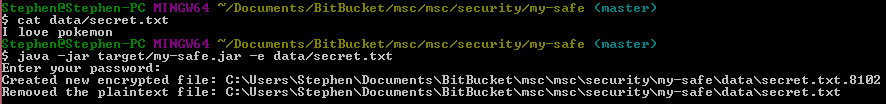
\includegraphics[width=0.9\linewidth]{images/safe_encrypt.png}
		\caption{Encryption}
		\label{fig:encryption}
	\end{figure}
	
	After the user has entered their password it will be hashed using SHA-256. It will then derive two keys from this hashed password; a 16-byte AES key and a 16-byte MAC key. These keys are digested further downstream. As the encryption uses AES-128 in CBC mode, an IV is required. Therefore the program creates a 16-byte IV using a \texttt{SecureRandom}, which generates cryptographically strong random numbers. 
	
	With the IV, AES key and plain text, the program is then free to generate the ciphertext. The cipher method is set to use AES in CBC mode and uses a PKC5 padding scheme. Finally, to provide message integrity (i.e. detecting tampering of the message, validating the password etc.), the program generates a 20-byte HMAC signature. The HMAC method combines the IV and ciphertext and hashes them using the SHA-1 hashing algorithm, with the MAC key used as input.
	
	The final step concatenates the 16-byte IV, ciphertext and 20-byte HMAC, encodes this value (Base64) and writes the value to file with a .8102 extension. The original plain text file is then deleted. The screenshot below shows the contents of the encrypted file:
	
	\begin{figure}[h!]
		\centering
		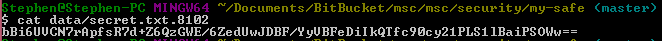
\includegraphics[width=0.9\linewidth]{images/safe_encrypted_data.png}
		\caption{Encryption data}
		\label{fig:encryptiondata}
	\end{figure}
	
	At no point in the program is the provided password stored as a String object. Java Strings are immutable and stored in a String pool for re-usability purposes - potentially for a long duration and therefore poses a security threat \cite{IEEEhowto:javastrings}.
	
	To decrypt the .8102 file and recover the original plain text file, the program can be run with the \texttt{-d [filename]} flag:
	
	\begin{figure}[h!]
		\centering
		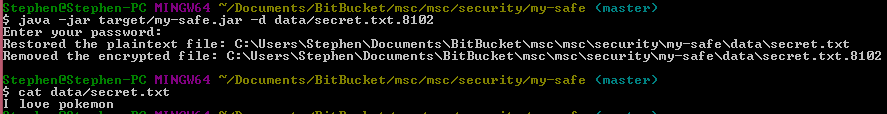
\includegraphics[width=0.9\linewidth]{images/safe_decrypt.png}
		\caption{Decryption}
		\label{fig:decryption}
	\end{figure}
	
	A password is again taken from the user and used to derive a MAC key. The program then reads the Base64 encoded string in the encrypted file and splits it into three parts; the first 16-bytes is the IV, the last 20-bytes is the HMAC and the remaining middle bytes is the ciphertext. As we have the original values used during encryption, we can take the new MAC key generated from the given password, along with the IV and ciphertext and generate a new HMAC. This new HMAC is then compared with the original HMAC from the encrypted message. 
	
	If the values differ then either the password supplied was incorrect or the message has been tampered with: 
	
	\begin{figure}[h!]
		\centering
		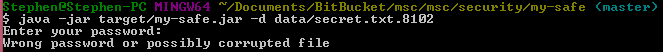
\includegraphics[width=0.9\linewidth]{images/safe_corrupted.png}
		\caption{Incorrect password or data corruption}
		\label{fig:corrupted}
	\end{figure}
	
	Otherwise the program will go ahead and decrypt the ciphertext, write the original plain text to a new file (without a .8102 extension) and delete the encrypted file.

	\subsection{Future Improvements}
	
	A key improvement to be made is that the program assumes any file ending with a .8102 extension is an encrypted file (and a file without this extension to be plain text). This poses two problems; firstly it allows a user to encrypt a file multiple times by manually adjusting the extension. Secondly, if this program  were to be packaged as a library to be included in other projects, the name of the extension should be configurable.
	
	Another improvement would be increasing the strength of the HMAC hashing algorithm. It is currently set to use SHA-1, however using SHA-256 would improve the strength of the signature. The performance penalty would be negligible for this kind of low throughput application.
	
	Finally, command line programs by nature, tend to be difficult to use and prone to keying errors. The core encryption \& decryption code could be put behind a graphical user interface (GUI) to improve usability
	
	\section{Hashed Password Cracking}\label{sec:hashcracking}
	
	The project enables a user to crack a given set of SHA-256 hashed passwords through a combination of dictionary attacks and brute force attacks. The dictionary is initially populated with prearranged case-insensitive strings, read from files in the \texttt{data/dictionary/} directory. 
	
	After the above strings have been exhausted from the dictionary, it then generates case-sensitive boy and girl names, each with a number between 1-9999 appended to it e.g. sOphiE654, JAck23. After these passwords are exhausted, the program will finally generate four-character, case-sensitive alphanumeric strings that can also contain special characters e.g. \$4Fc, H\&1*. 
	
	We are given some initial clues about the hashed passwords:
	
	\begin{enumerate}
		\item A lower-case first name among the 10 most popular girl names in England.
		\item A lower-case first name among the 10 most popular boy names in England.
		\item A name, as specified in the dictionaries of 1 and 2, but with no specified case and with a number up to 9999 at the end.
		\item A lower-case English word.
		\item A combination of 4 alphanumerical characters, with no specified case, and with special characters.
	\end{enumerate}
	
	The program requires three command line arguments; an input file (\texttt{-i [filename]}) containing the list of hashes to be cracked, an output file (\texttt{-o [filename]}) where the results will be written to and lastly, the location of the directory containing the dictionary files (\texttt{-d [directory]}). 
	
	Failure to supply any of the above arguments (or a file does not exist) will terminate the program. Before the program attempts to crack any hashes, an output file will be created (if it didn't already exist) or the contents of an already existing output file will be deleted.
	
	During runtime, any cracked hash is immediately piped to the output file as a newline in the format of \texttt{[hash password]}. The program will take less than a minute to complete.
	
	See the projects \texttt{README.md} file for more detailed run instructions.
	
	\subsection{Implementation}
	
	A metrics object is first created to keep track of various measurements such as execution time and the count of generated test passwords. The program then enters it's main loop and attempts to crack all eight provided SHA-256 hashed passwords. The main loop will break if either all hashes are solved or the dictionary is fully exhausted.
	
	In each iteration, a generated password is polled from the dictionaries current password queue. This password is then hashed down using SHA-256 ready for comparison. The hashes stored in the input file are hexadecimal values, therefore the program uses a \texttt{DatatypeConverter} to parse the hex value so the bytes can be compared.
	
	If the generated hash value matches a hash from the input file, it will write the original hash and parsed plain text value to the output file.
	
	Most of the programs complexity resides in updating the dictionaries password queue at runtime, specifically when attempting to solve for rules 3 and 5 above. 
	
	When generating passwords for rule 3, the possible number of case-insensitive numeric combinations for each name is \texttt{$2^{n}*10000$}, where \texttt{n} equals the names length. To avoid memory issues, one call only generates 10,000 password results which correspond to one name permutation e.g. \texttt{[sOphie1, sOphie2, ..., sOphie9999]}.
	
	Generating passwords to satisfy the final rule is a true brute force attack. The algorithm uses a recursive method to generate all possible four character combinations from a given 71 character long alphabet. Initially, this method generated every four letter combination atomically. However, it quickly ran into memory issues due to the \texttt{$71^{4}$} complexity and created a lot of redundant processing cycles. 
	
	To mitigate this, the algorithm was altered to generate and cache all three letter password combinations (a much smaller \texttt{$71^{3}$} problem). Then, each subsequent call polls a three letter password from the cache, loops through the alphabet and appends each letter to the password. Therefore each call only returns 71 new passwords at a time.
	
	Both of the above algorithms have been optimised to avoid redundant processing and minimise memory consumption.	
	
	Pre-optimisation, the project successfully solved all eight hashes in 31.829 seconds and generated approximately 34 million test passwords. Therefore the output file contains the following data after execution:
	
	\begin{itemize}
		\item \texttt{5E0176C...} \texttt{sophie}
		\item \texttt{B9DD960...} \texttt{charlie}
		\item \texttt{D813086...} \texttt{JeSsicA42}
		\item \texttt{FFFF0E6...} \texttt{haRRY1980}
		\item \texttt{AB8A711...} \texttt{inoepithelioma}
		\item \texttt{4ABB806...} \texttt{unbreakable}
		\item \texttt{20ABFE9...} \texttt{K4t!}
		\item \texttt{20D9787...} \texttt{@c3*}
	\end{itemize}

	Console output of the generated metrics after execution are shown below:
	
	\begin{figure}[h!]
		\centering
		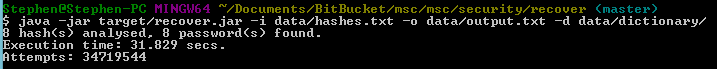
\includegraphics[width=0.9\linewidth]{images/recover_pre_optimised.png}
		\caption{Pre-optimised console output}
		\label{fig:preoptimisedconsoleoutput}
	\end{figure}	

	\subsection{Post-optimisation}
	
	To simulate the danger and effect of an attacker only knowing the first letter of your password (perhaps through shoulder surfing), the internal alphabet array was slightly modified so that the '@' and 'K' characters are at the start of the alphabet. After this small change, all hashed passwords were found in 14.829 seconds and only generated approximately 13 million test passwords.
	
	\begin{figure}[h!]
		\centering
		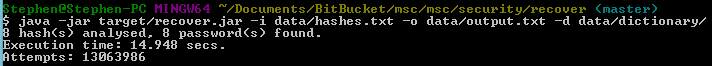
\includegraphics[width=0.9\linewidth]{images/recover_post_optimised.png}
		\caption{Post-optimised console output}
		\label{fig:postoptimisedconsoleoutput}
	\end{figure}
	
	\subsection{Future Improvements}
	
	Ideally, in a real world situation, the dictionary size would need to be much larger. The problem however, is that the larger the pool gets, the memory and time demands also rise exponentially. The processing time of generating and hashing passwords could potentially be parallelised through multi-threading to help mitigate some of the cost.
	
	However, the main lesson to take away from this program is that targeted attacks (i.e. when an attacker may have additional information on the victim) drastically reduces security. The small post-optimisation shown above actually led to a 47\% reduction in execution time and generated 38\% less test passwords.
	
	Again, similar to the encryption \& decryption program, a GUI to analyse the results would improve usability.
	
	% references section
	
	\begin{thebibliography}{1}
		
		\bibitem{IEEEhowto:javastrings}
		Docs.oracle.com. (2017). Java Cryptography Architecture (JCA). [online] Available at: https://docs.oracle.com/javase/6/docs/technotes/ guides/security/crypto/CryptoSpec.html\#PBEEx [Accessed 14 Dec. 2017]

	\end{thebibliography}

\end{document}